\documentclass{PoS}
\usepackage{xspace}

\title{Measurements of Vector boson fusion with the ATLAS detector}

\ShortTitle{Measurements of Vector boson fusion with the ATLAS detector}

\author{\speaker{Kurt Brendlinger},
        on behalf of the ATLAS Collaboration\\
%%         \thanks{A footnote may follow.}\\
       Deutsches Elektronen-Synchrotron (DE)\\
       E-mail: \email{kurt.brendlinger@cern.ch}}

%\author{Another Author\\
%        Affiliation\\
%        E-mail: \email{...}}

\abstract{The ATLAS experiment with data collected by the Large Hadron Collider (LHC).}

\FullConference{The European Physical Society Conference on High Energy Physics\\
                 5-12 July\\
                 Venice, Italy}

\begin{document}
\def\wjj{\ensuremath{W\kern -0.2em j\kern -0.1emj}\xspace}
\def\zjj{\ensuremath{Z\kern -0.1em j\kern -0.1emj}\xspace}

This talk presented stuff from the ATLAS detector \cite{Aad:2008zzm} collected by the
LHC \cite{Evans:2008zzb}.
The first result presented is a measurement of the \wjj production \cite{Aaboud:2017fye}.
The second result is a \zjj result.

\section{\wjj Production Measurement}

Figure~\ref{wjj-cartoons}.

\begin{figure}
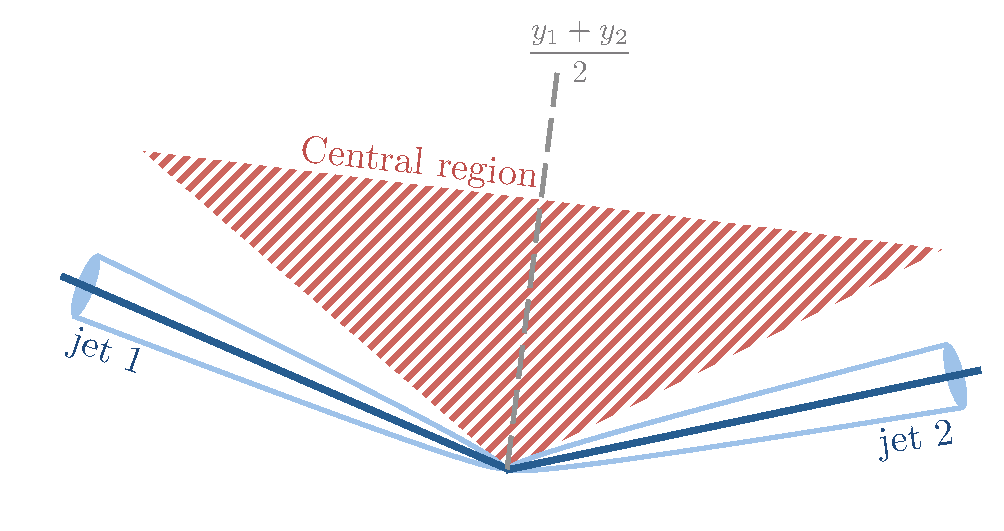
\includegraphics[width=.49\textwidth]{STDM-2014-11/fig_03.pdf}
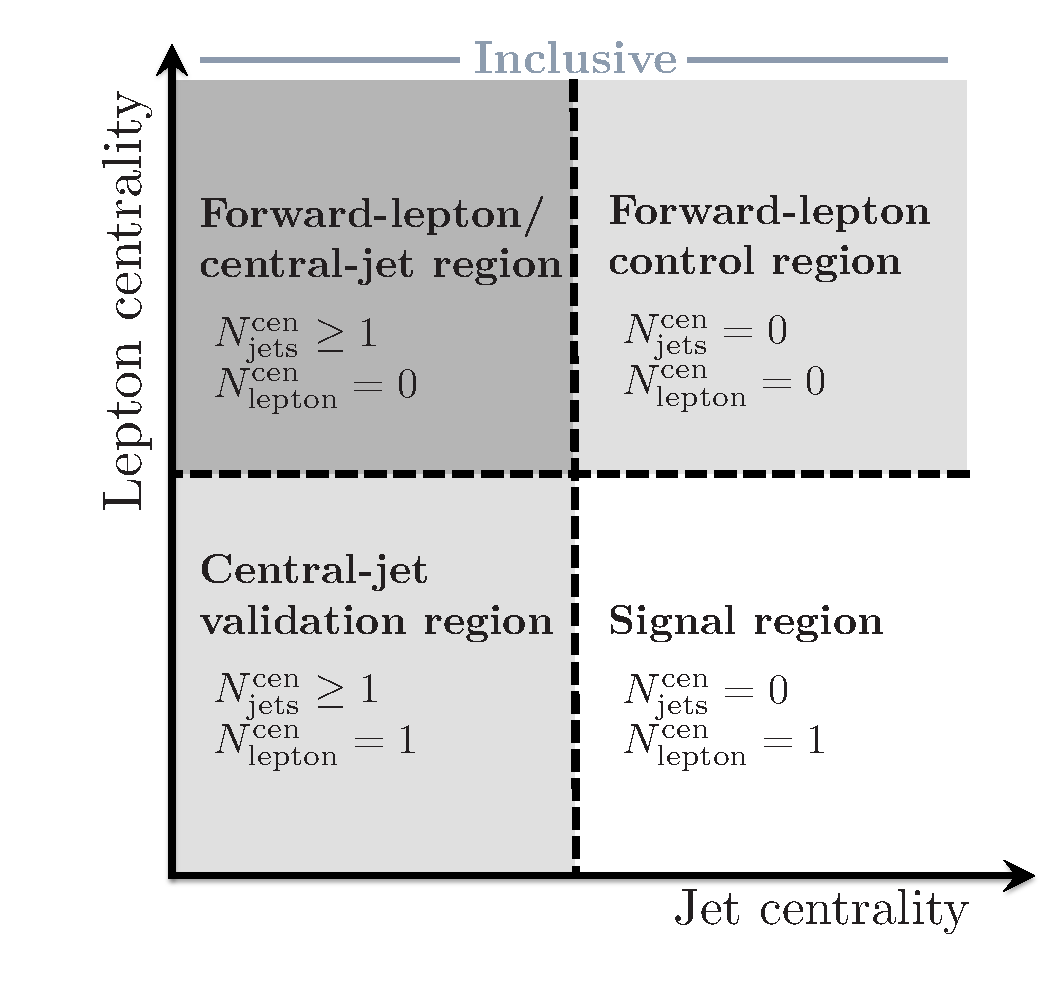
\includegraphics[width=.49\textwidth]{STDM-2014-11/fig_04.pdf}
  \caption{Left: Depiction of...}
  \label{wjj-cartoons}
\end{figure}

Figure~\ref{wjj-discriminating-variables}.

\begin{figure}
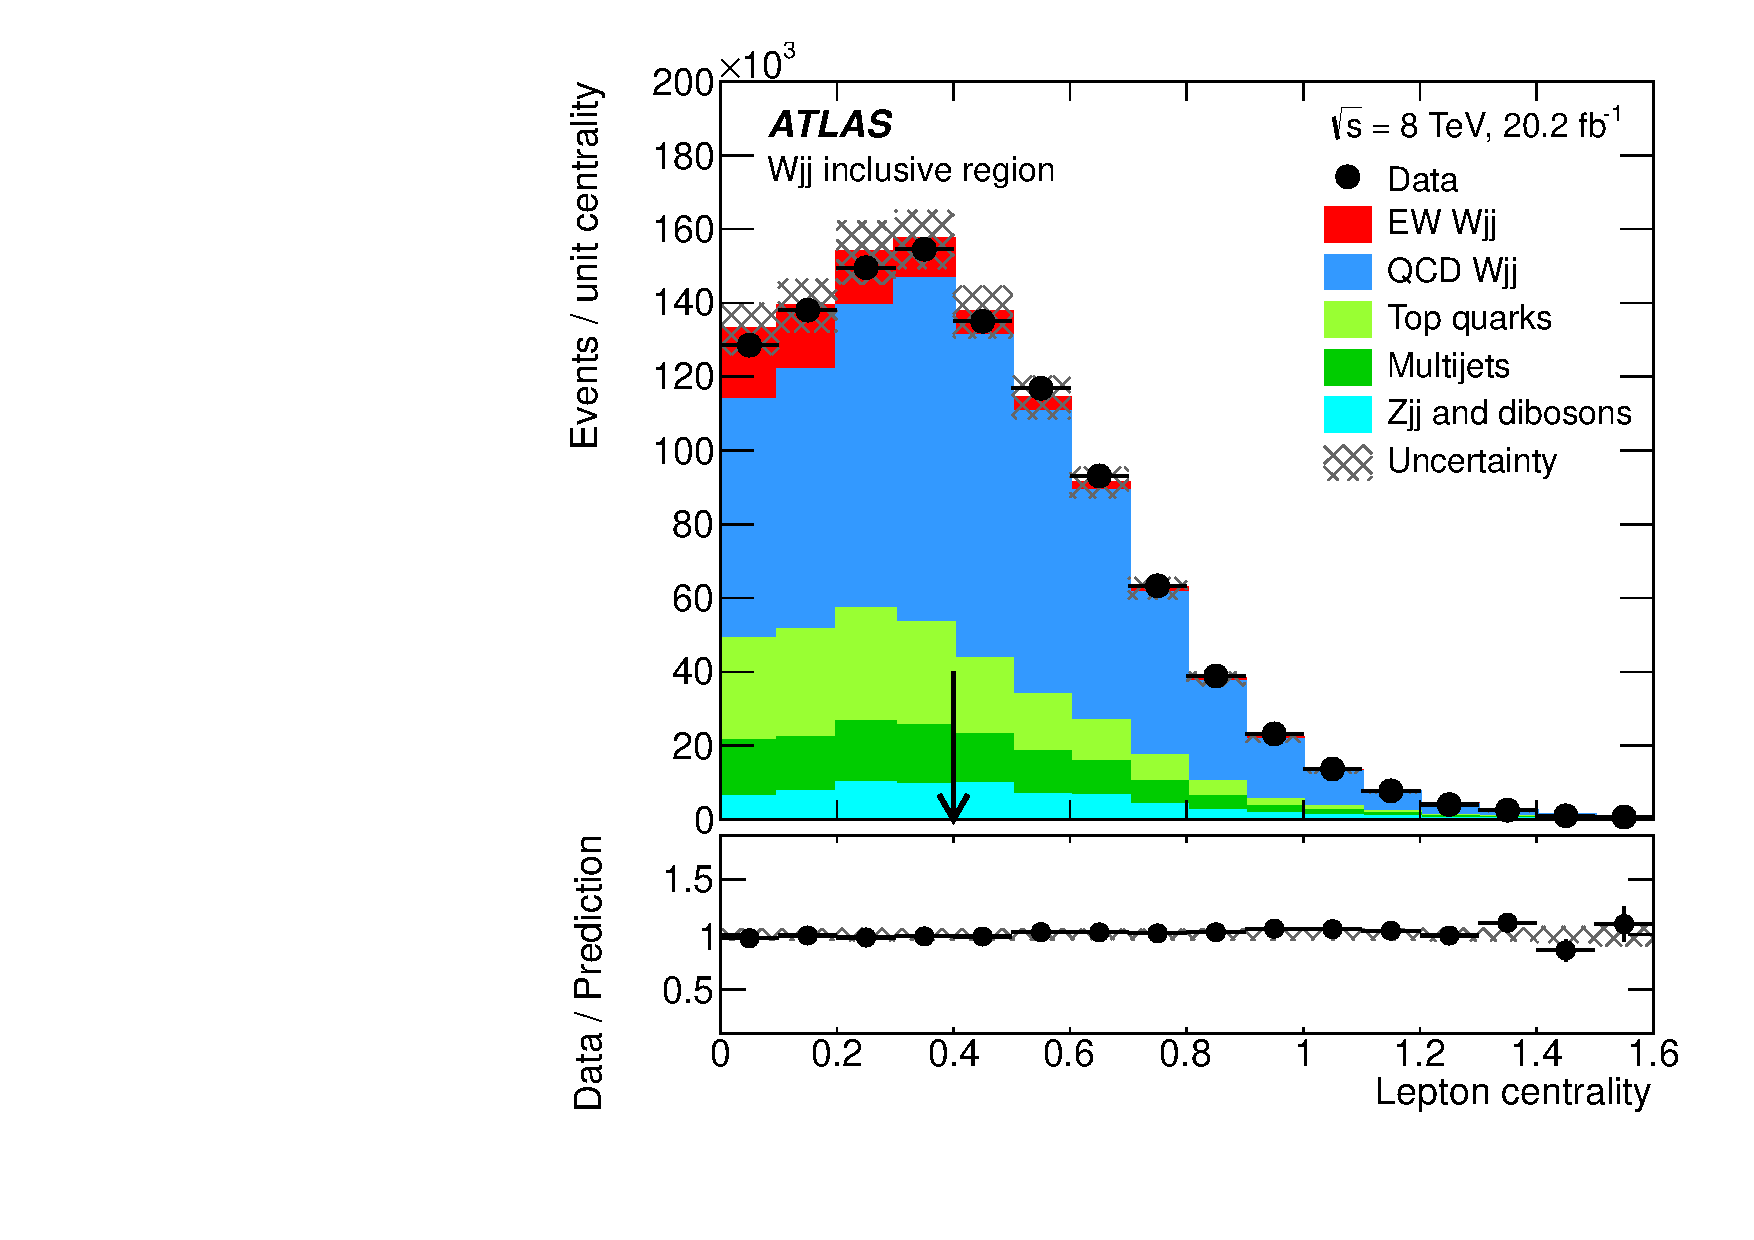
\includegraphics[width=.49\textwidth]{STDM-2014-11/fig_05b.pdf}
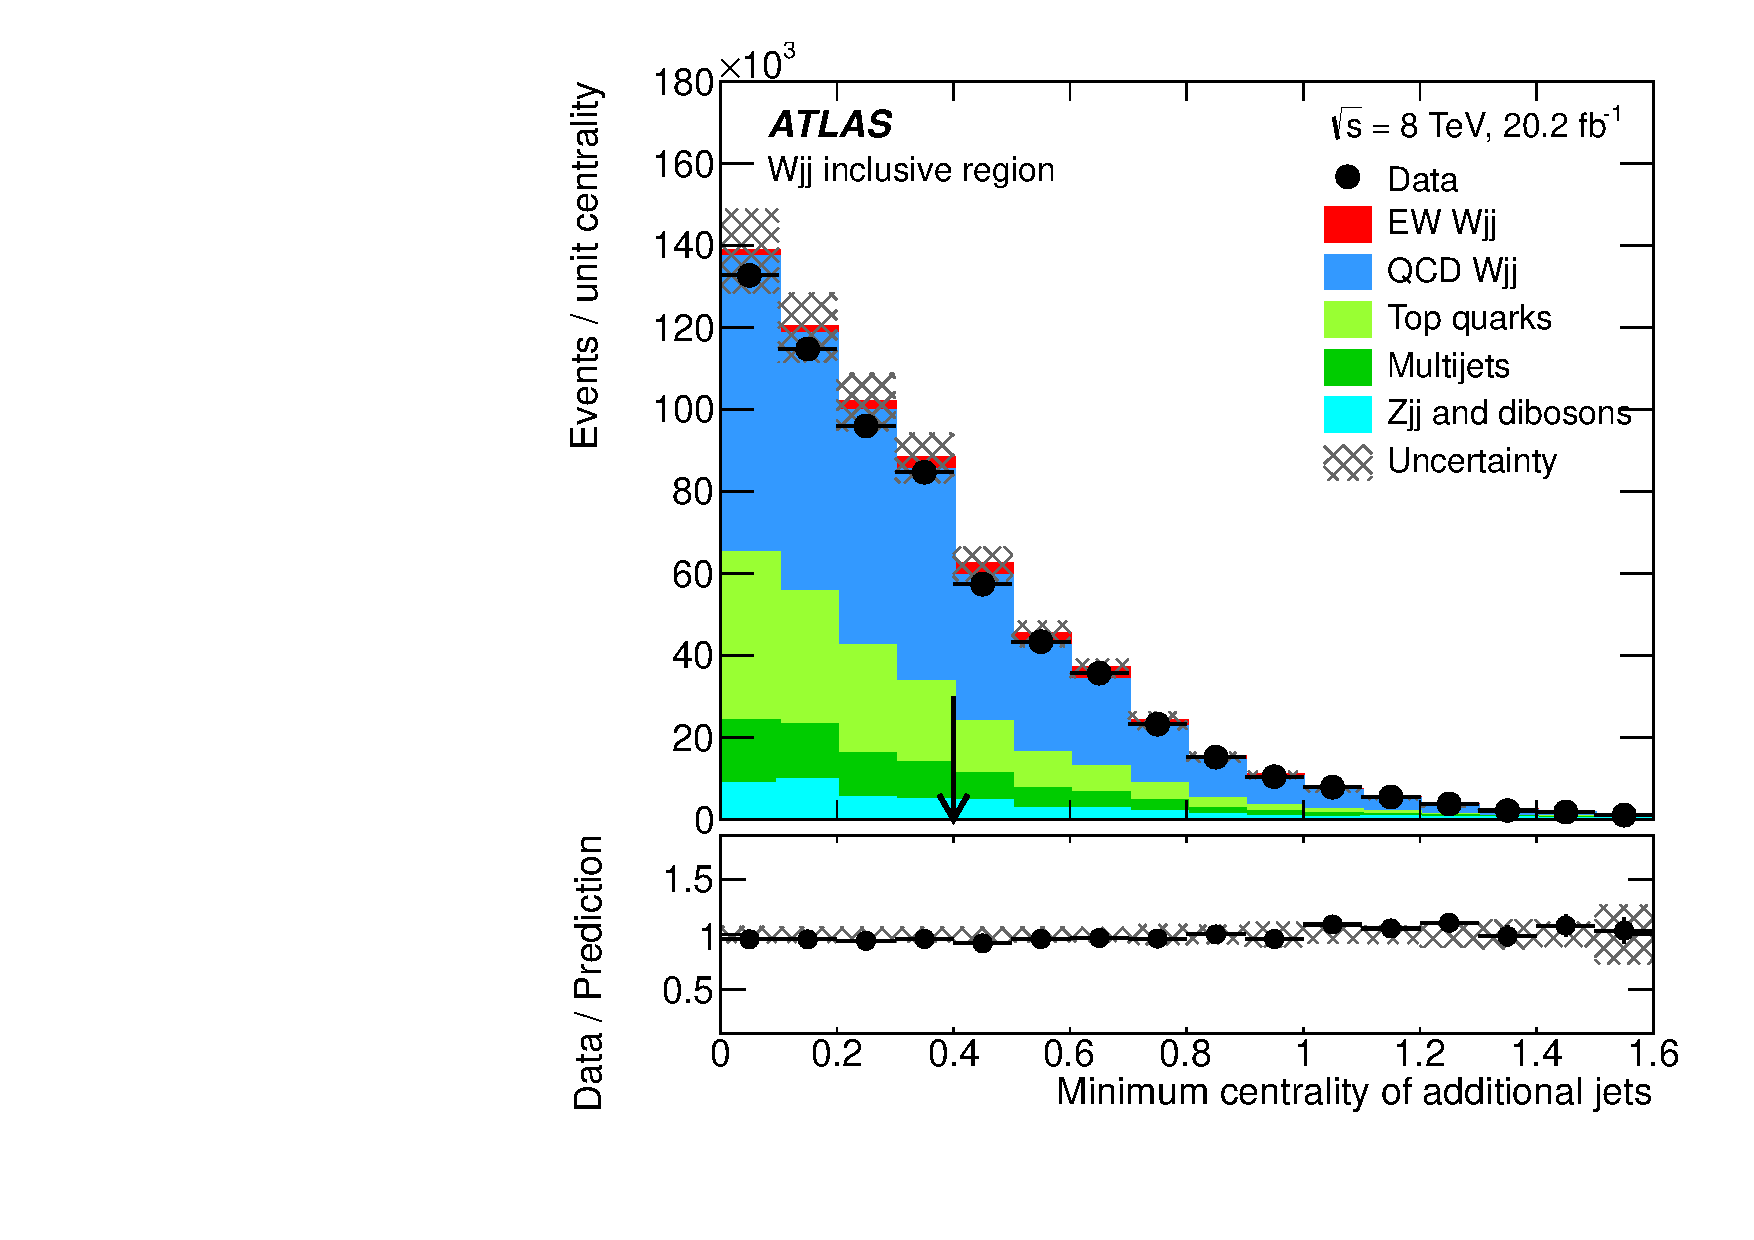
\includegraphics[width=.49\textwidth]{STDM-2014-11/fig_05d.pdf}
  \caption{Discriminating variables.}
  \label{wjj-discriminating-variables}
\end{figure}

Figure~\ref{wjj-mjj-distribution}.

\begin{figure}
  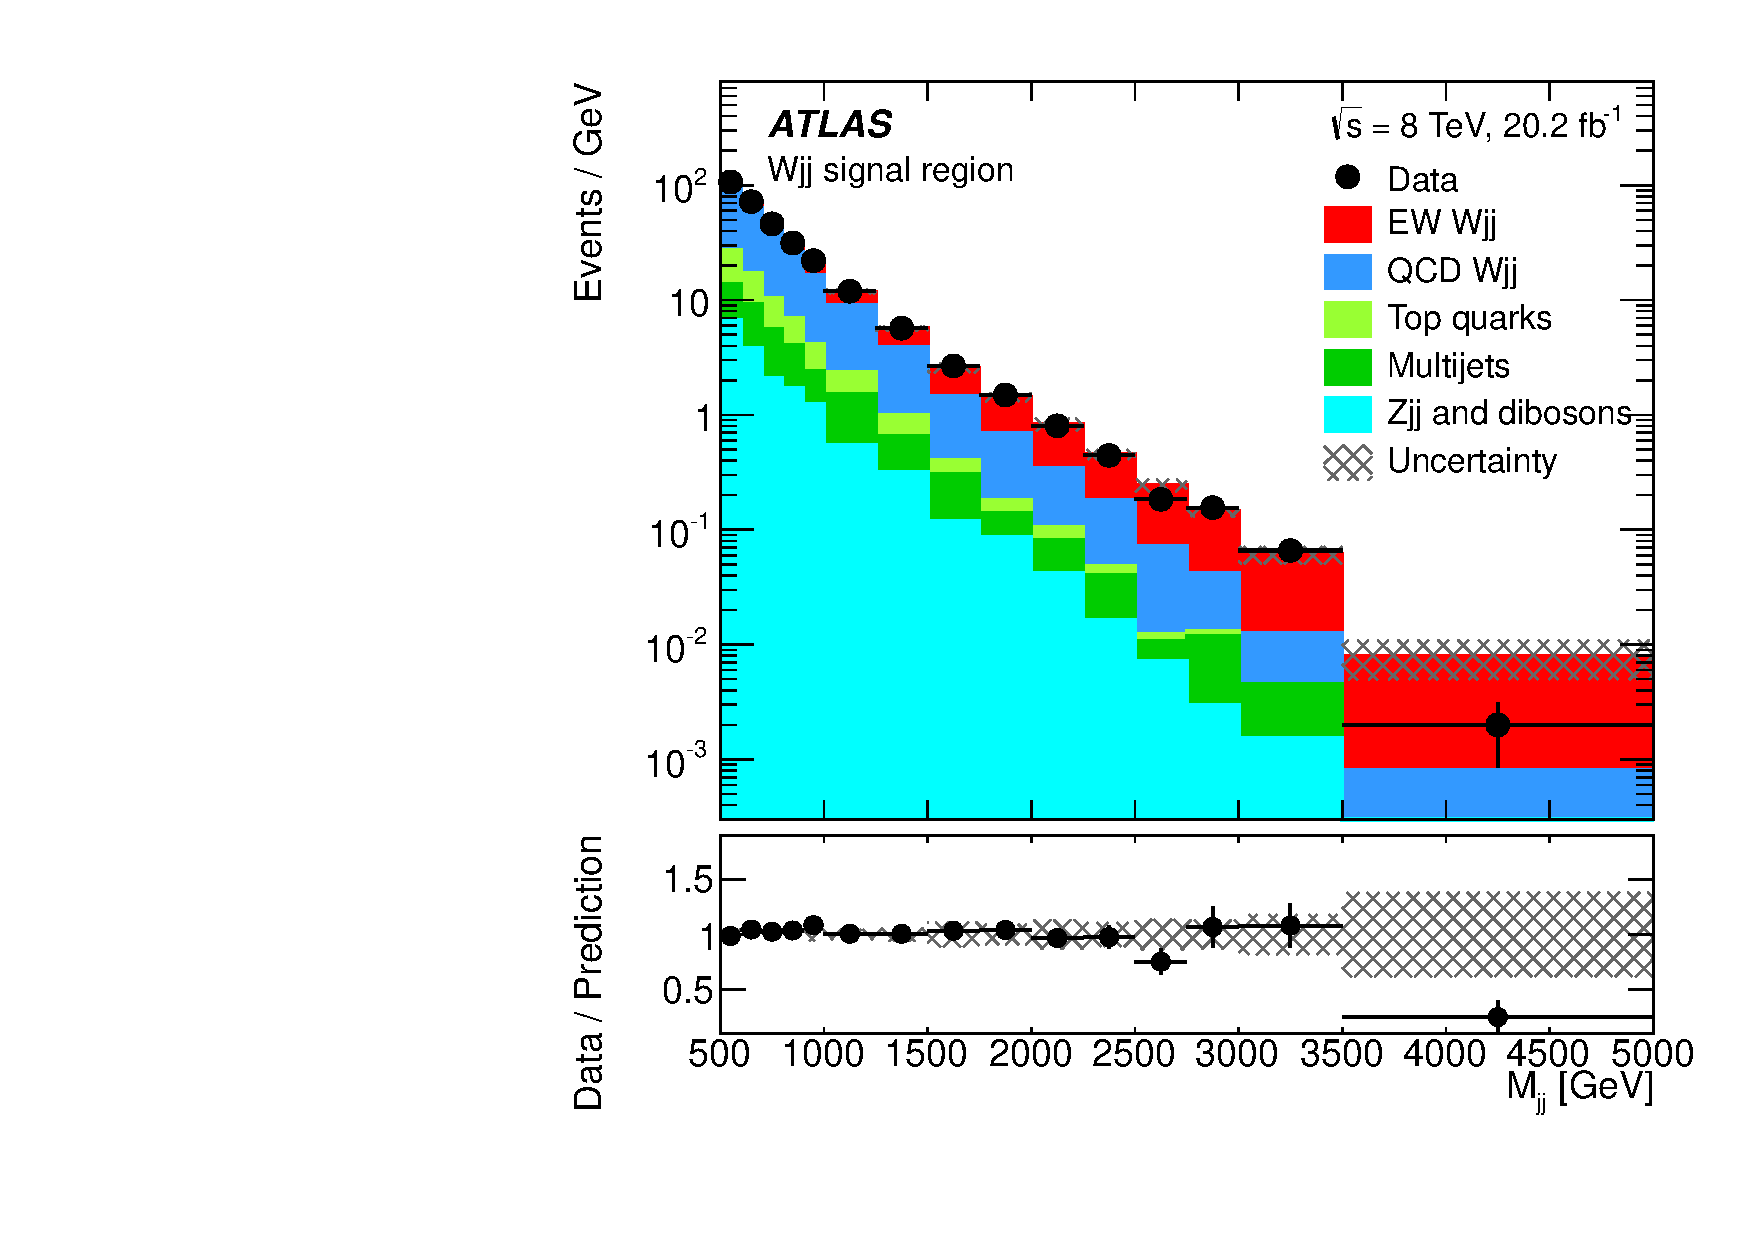
\includegraphics[width=.49\textwidth]{STDM-2014-11/fig_09b.pdf}
  \caption{The $m_{jj}$ distribution.}
  \label{wjj-mjj-distribution}
\end{figure}

Figure~\ref{wjj-differential-distributions}.

\begin{figure}
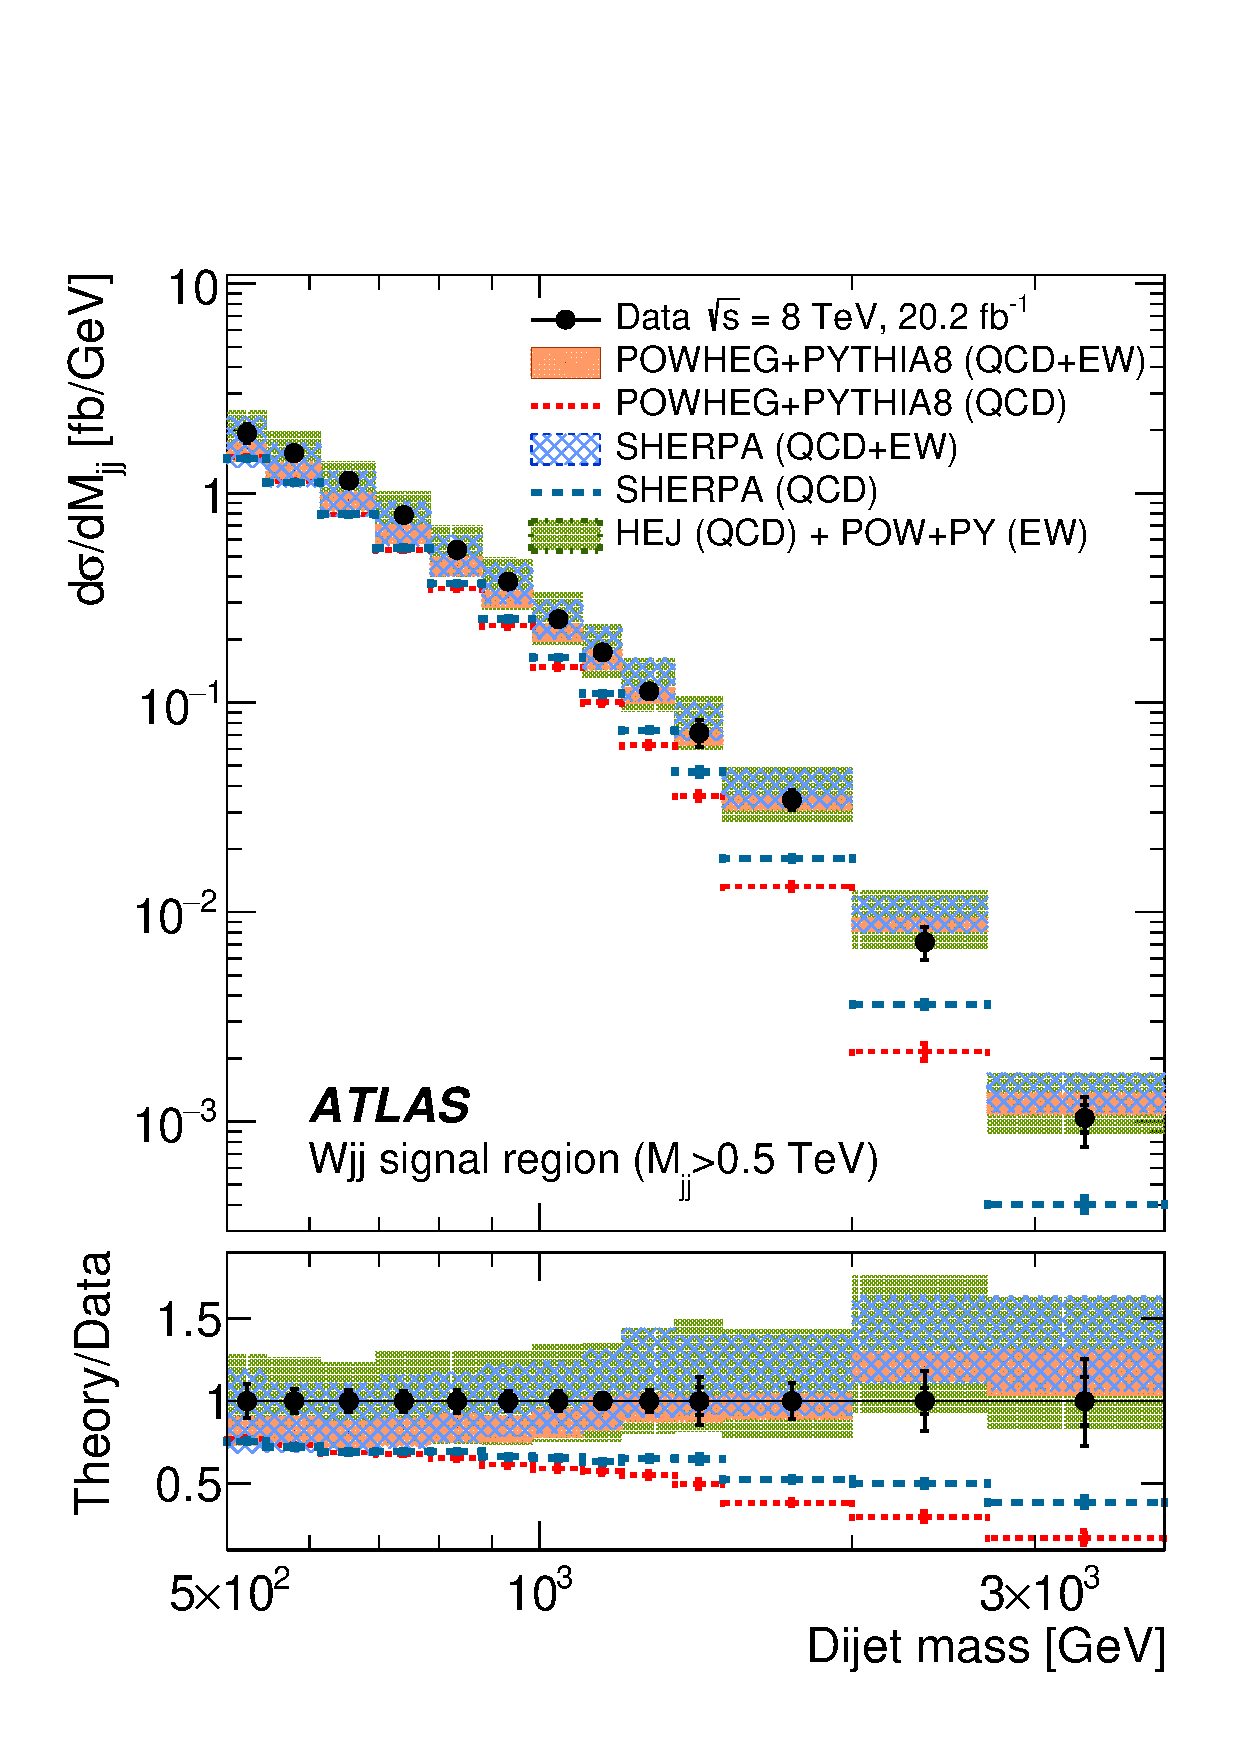
\includegraphics[width=.49\textwidth]{STDM-2014-11/fig_16a.pdf}
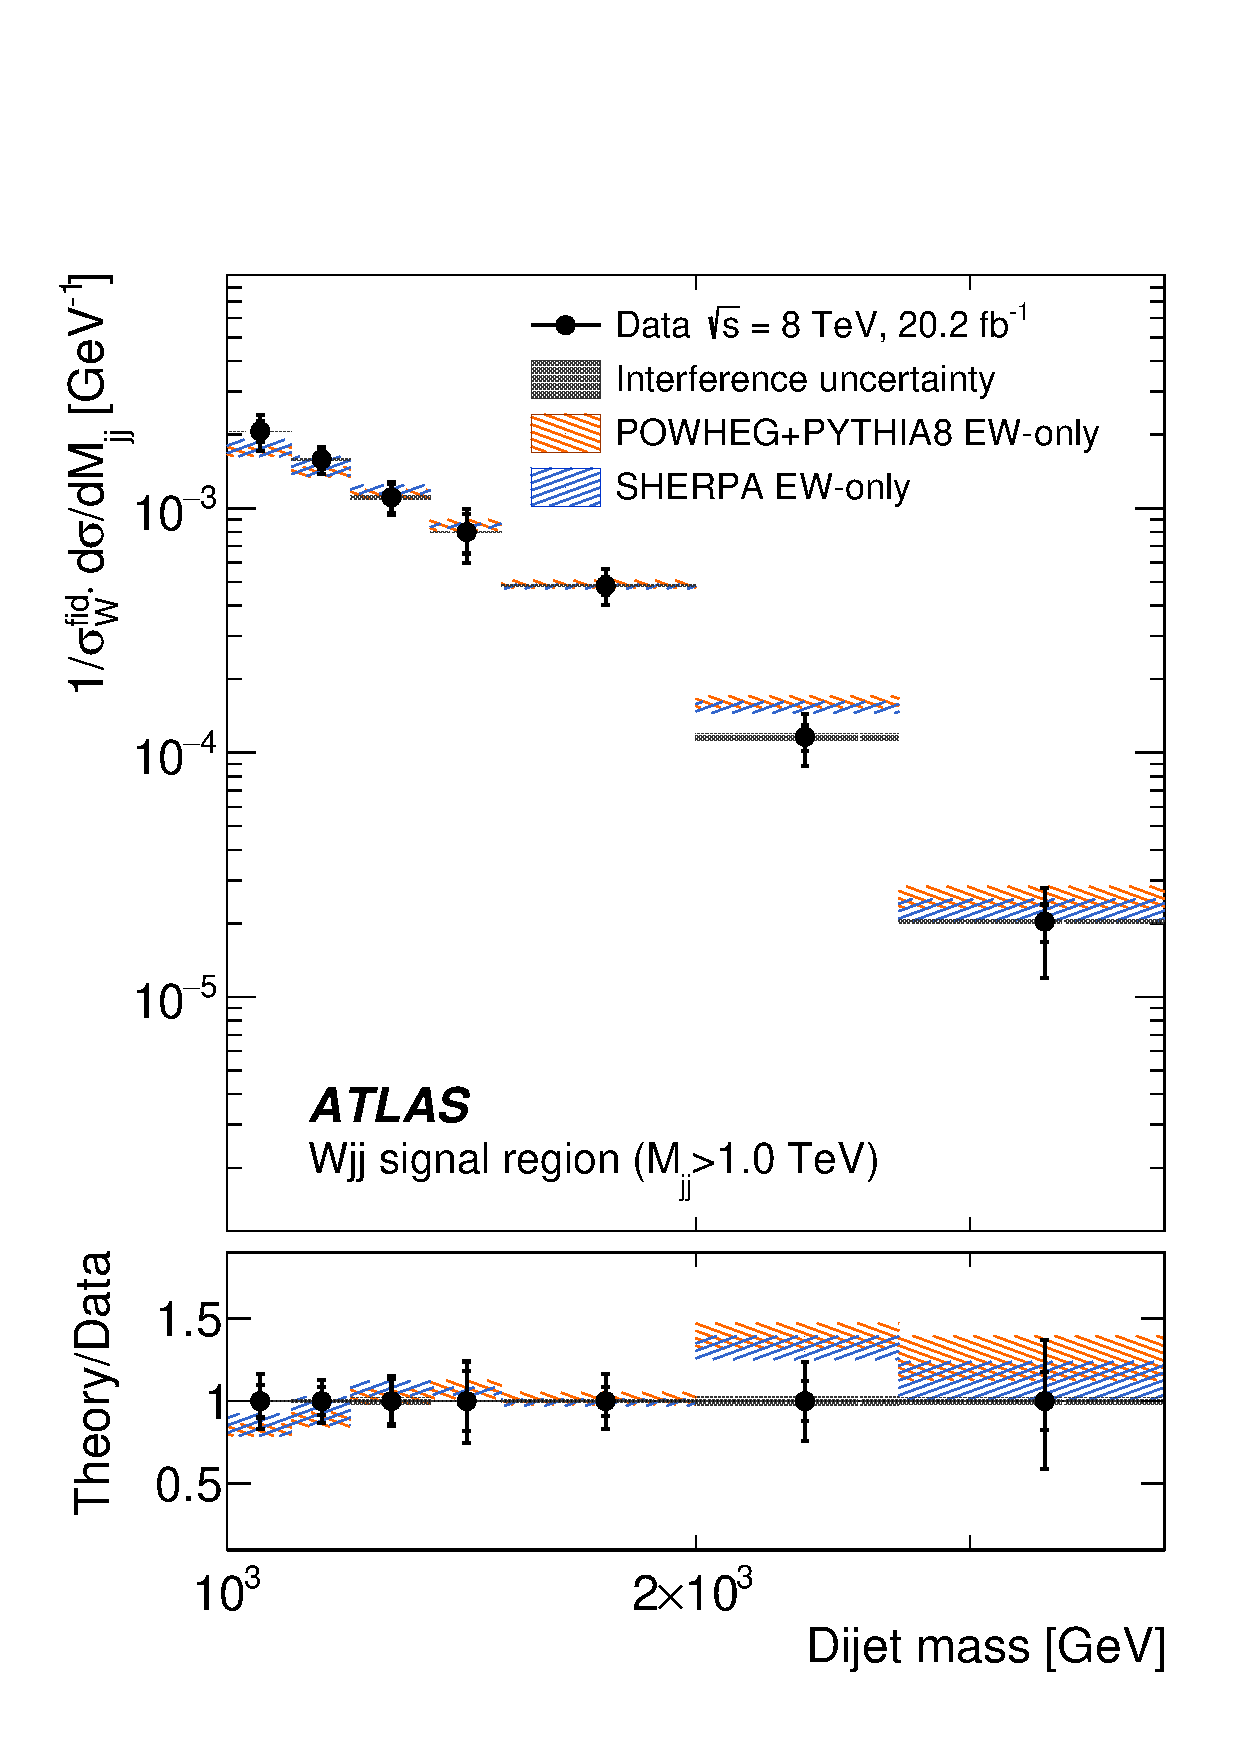
\includegraphics[width=.49\textwidth]{STDM-2014-11/fig_19b.pdf}
  \caption{Differential Distributions.}
  \label{wjj-differential-distributions}
\end{figure}

Figure~\ref{wjj-atgc}.

\begin{figure}
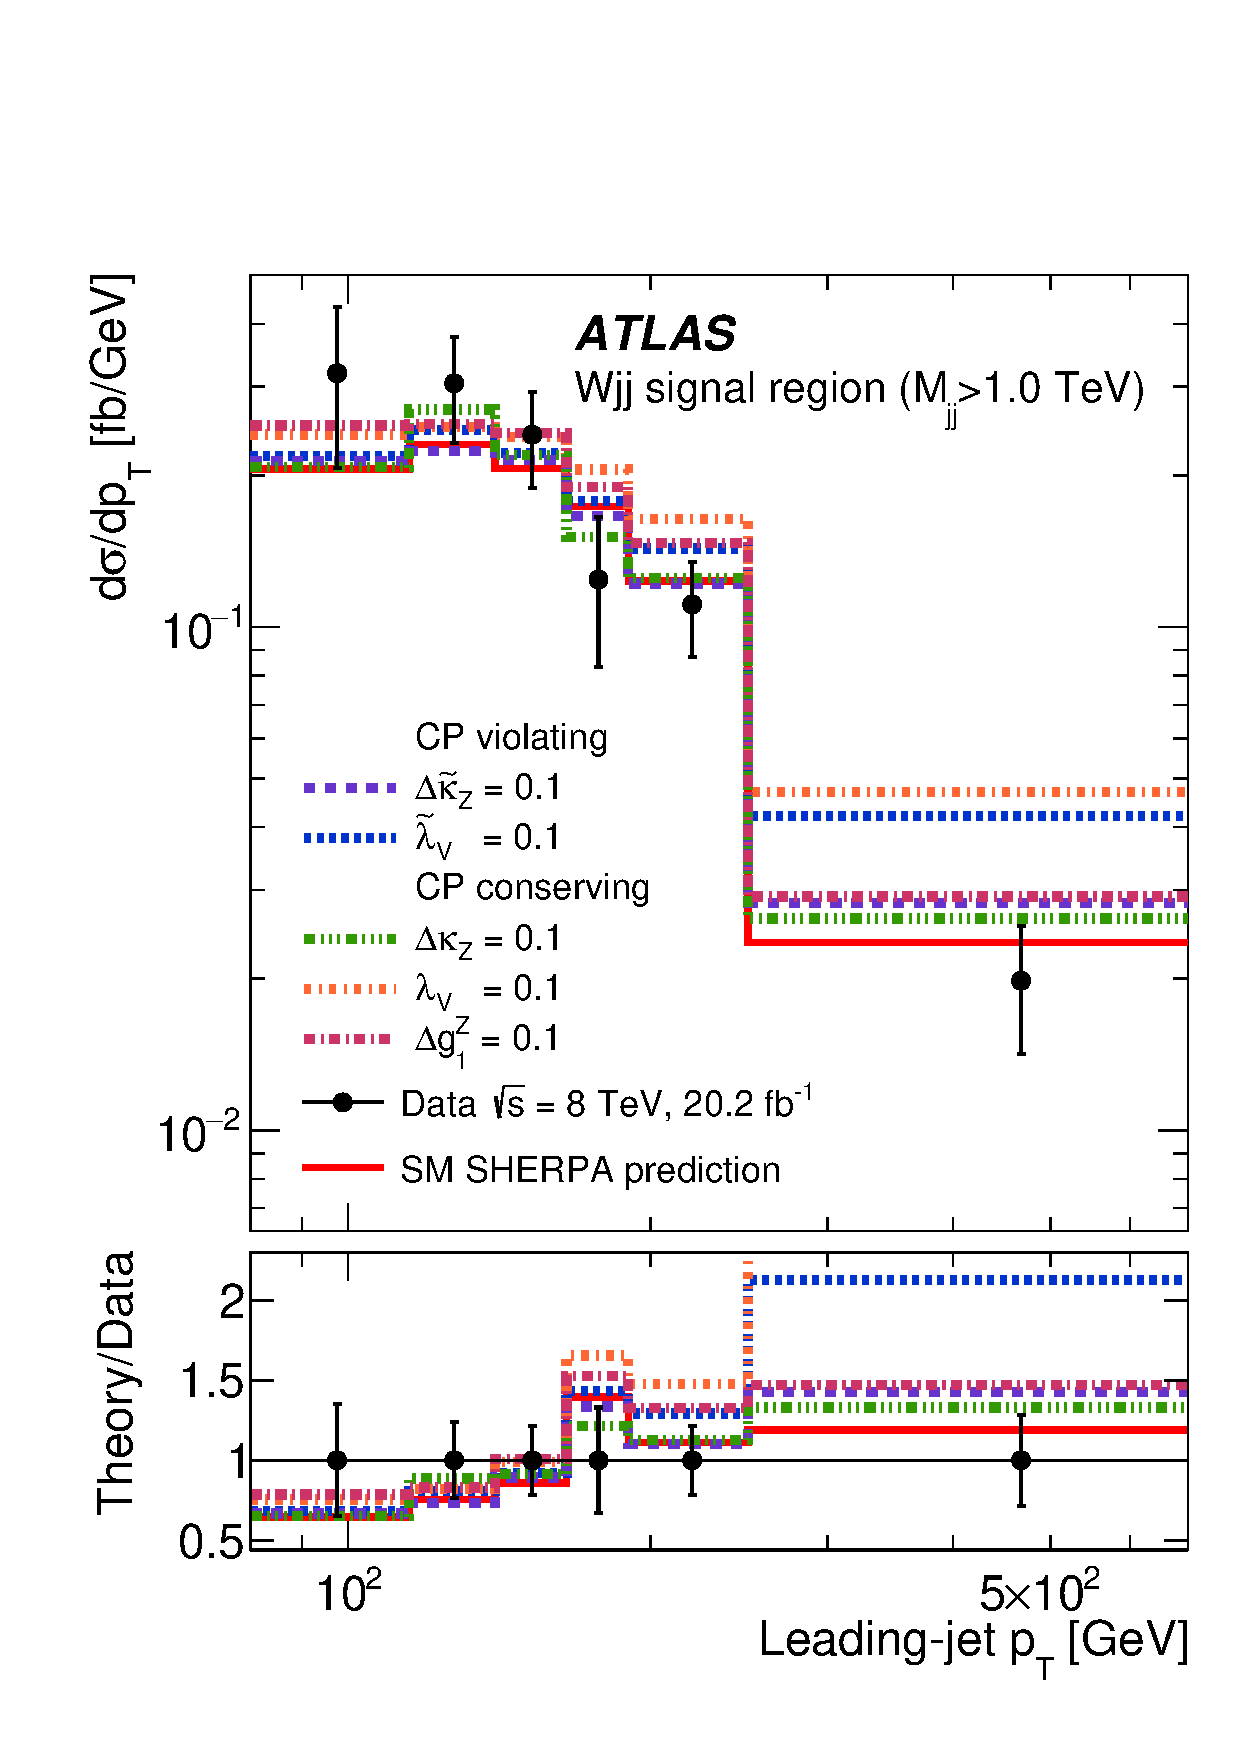
\includegraphics[width=.49\textwidth]{STDM-2014-11/figaux_30b.pdf}
  \caption{Anomalous triple gauge couplings.}
  \label{wjj-atgc}
\end{figure}

%% \begin{figure}
%% 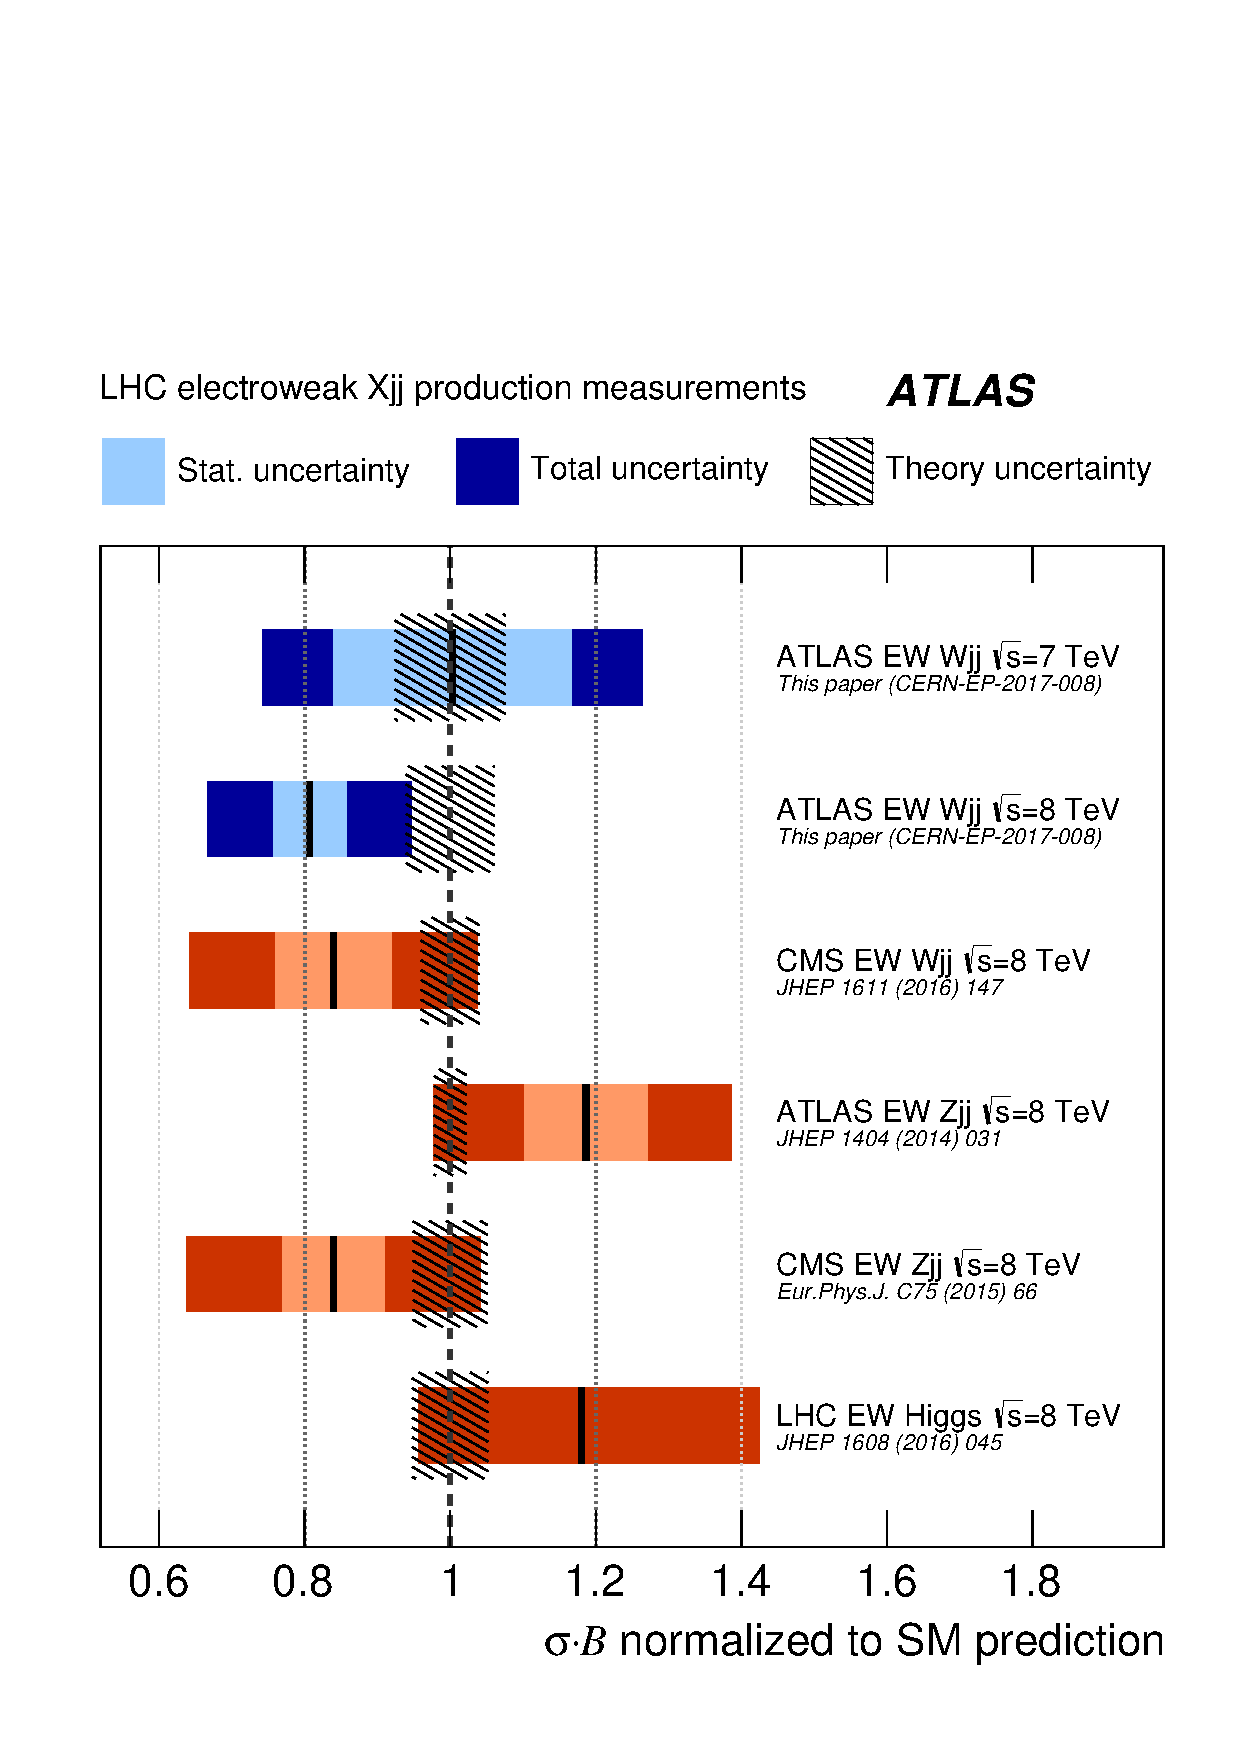
\includegraphics[width=.49\textwidth]{STDM-2014-11/fig_10.pdf}
%%   \caption{LHC electroweak Xjj production measurments (according to the 8 TeV paper).}
%%   \label{wjj-summary}
%% \end{figure}



\section{\zjj Production Measurement}

Figure~\ref{zjj-dijet-mismodeling} describes blah.

\begin{figure}
  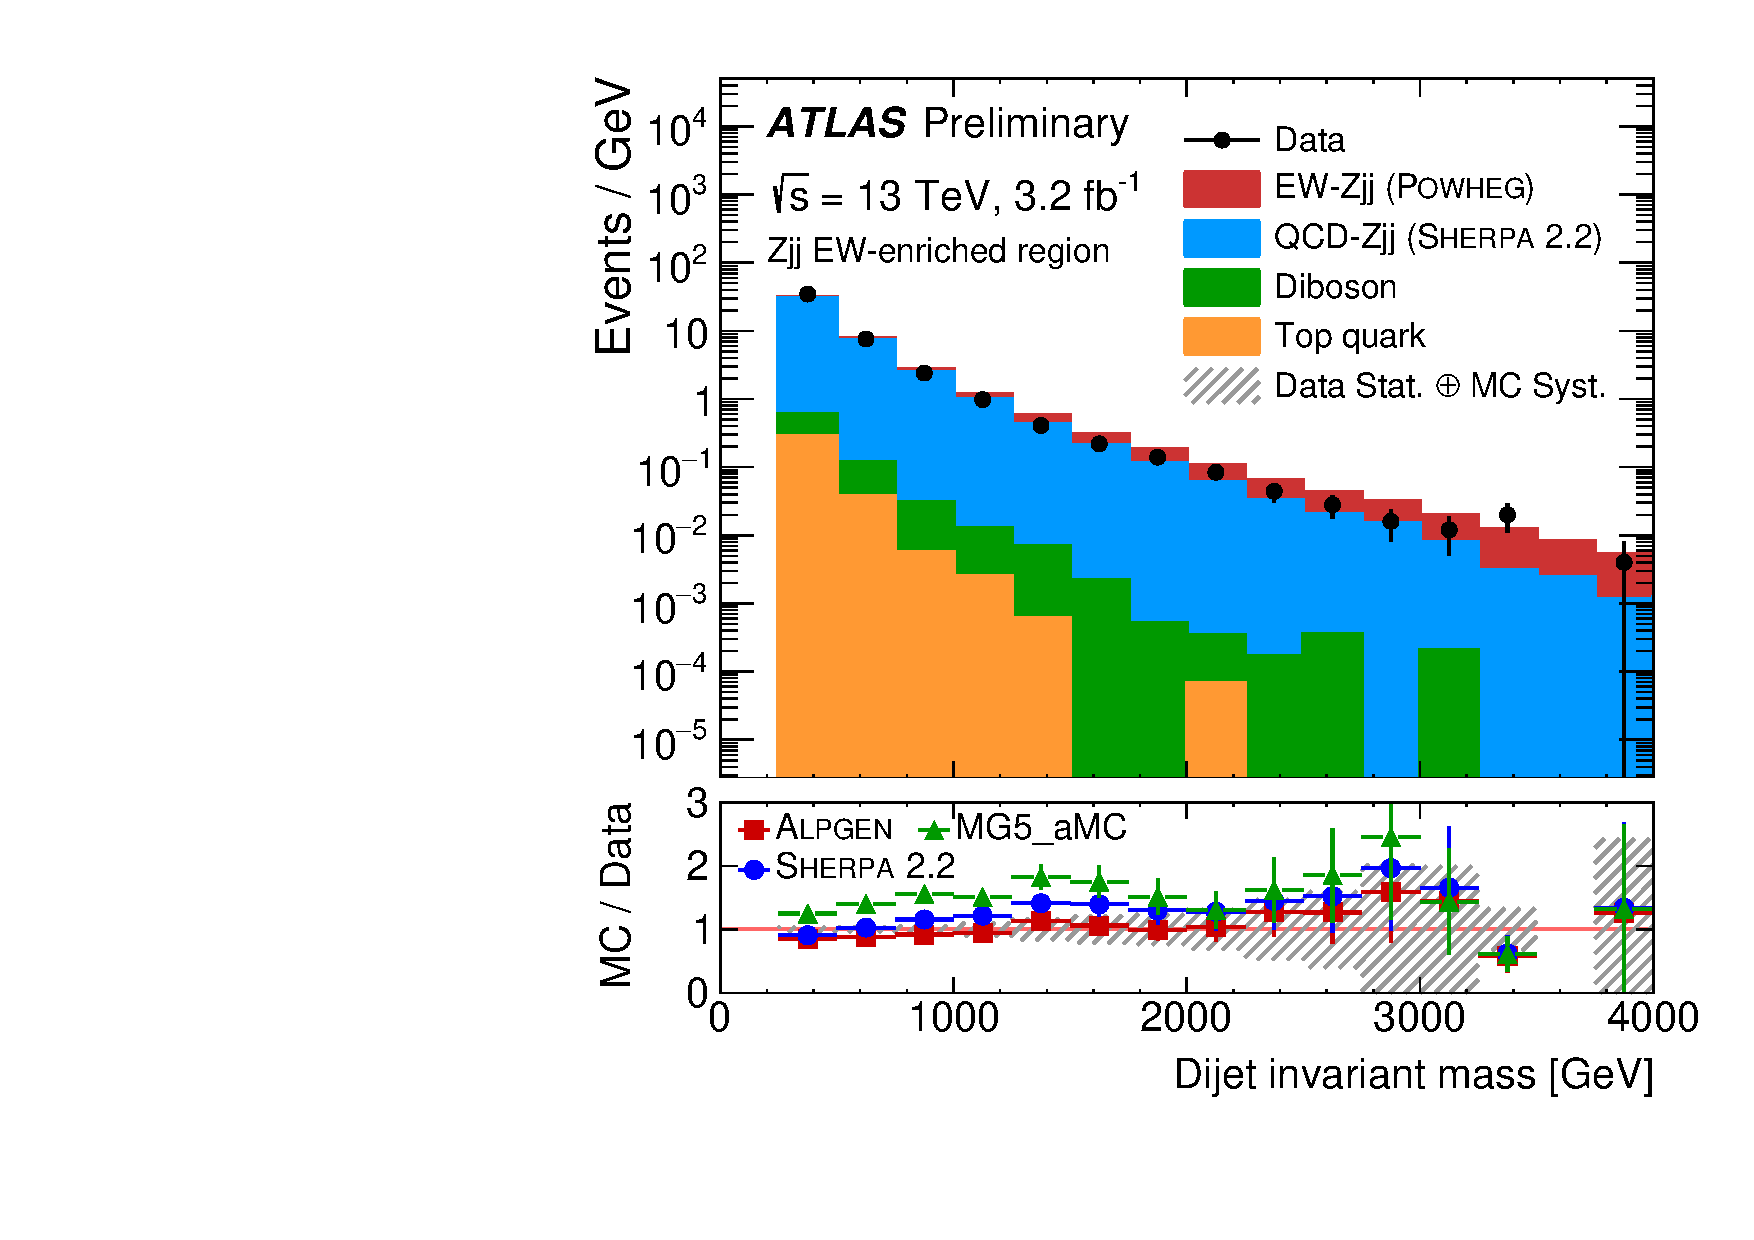
\includegraphics[width=.33\textwidth]{STDM-2016-09/fig_02a.pdf}
  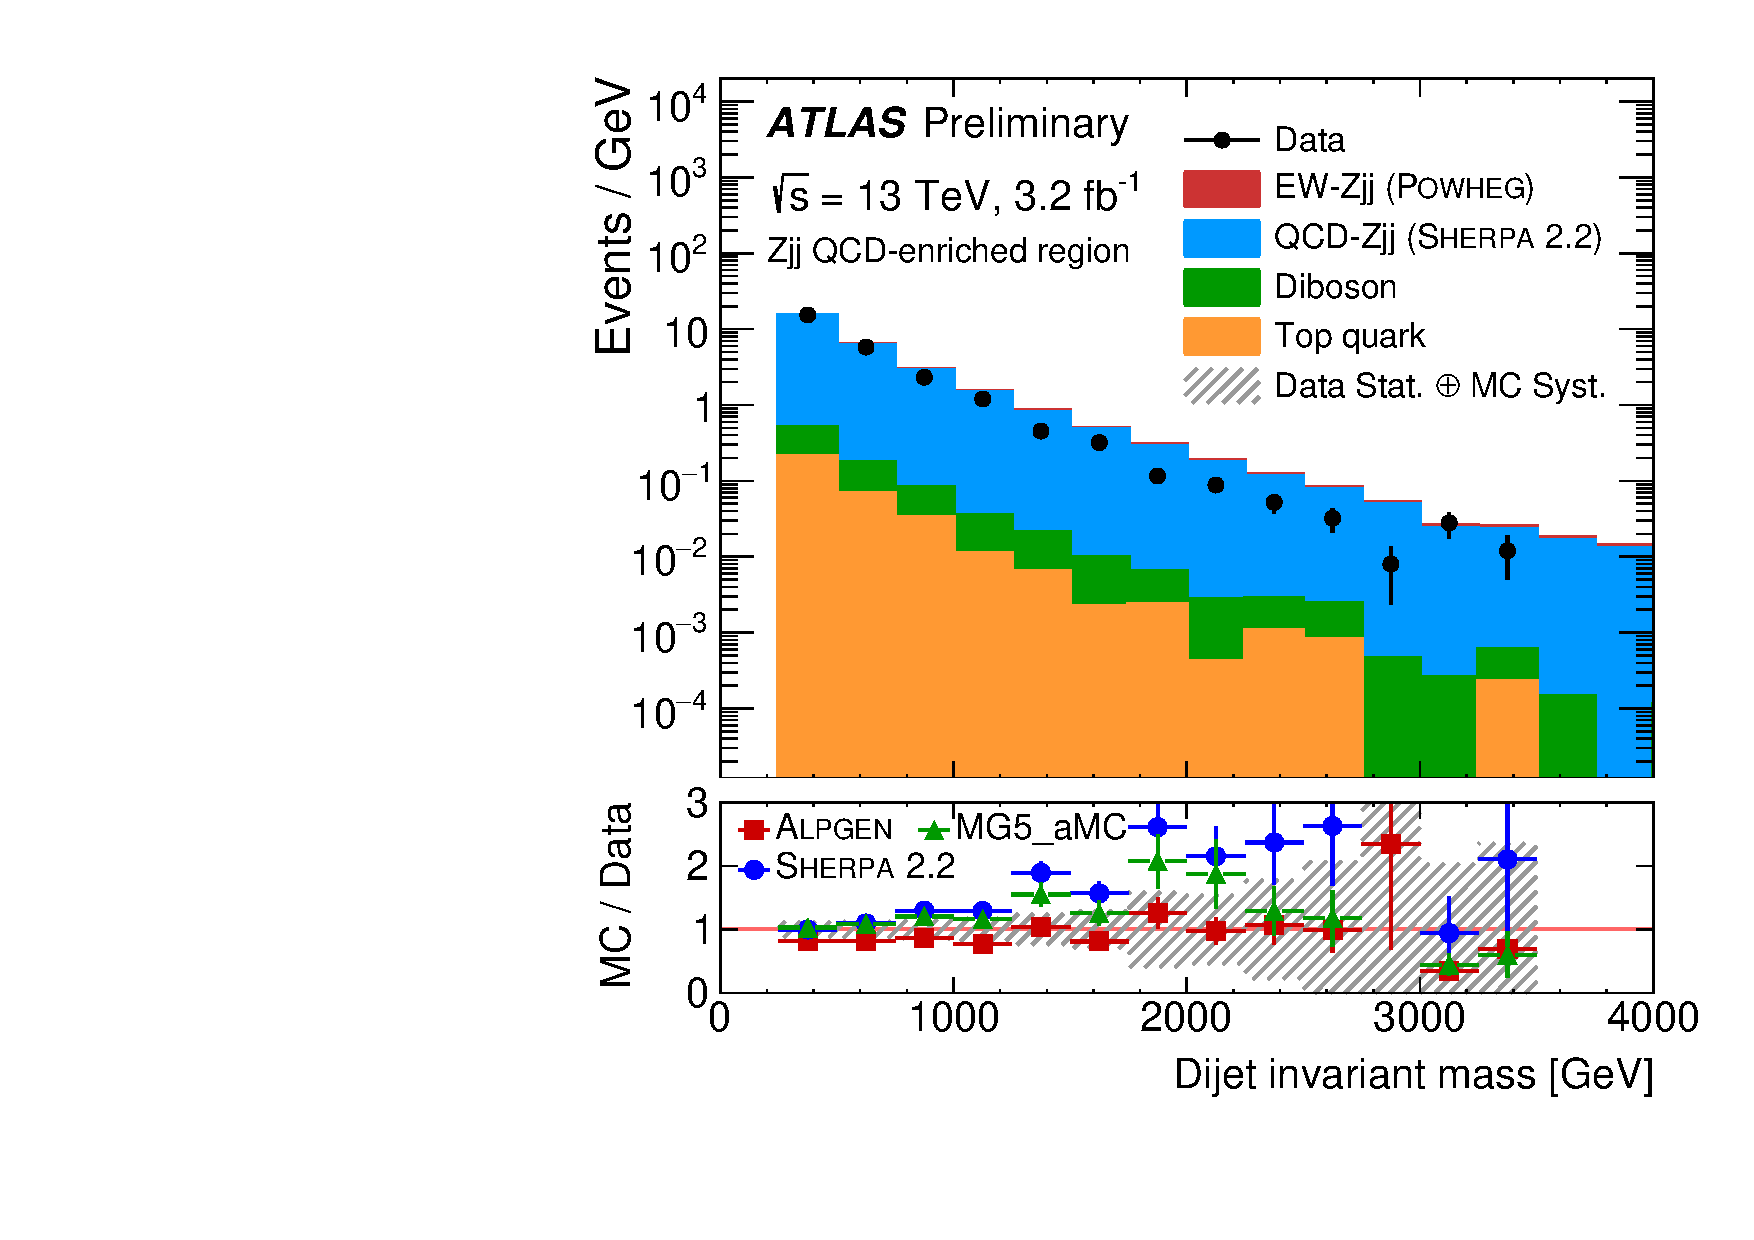
\includegraphics[width=.33\textwidth]{STDM-2016-09/fig_02b.pdf}
  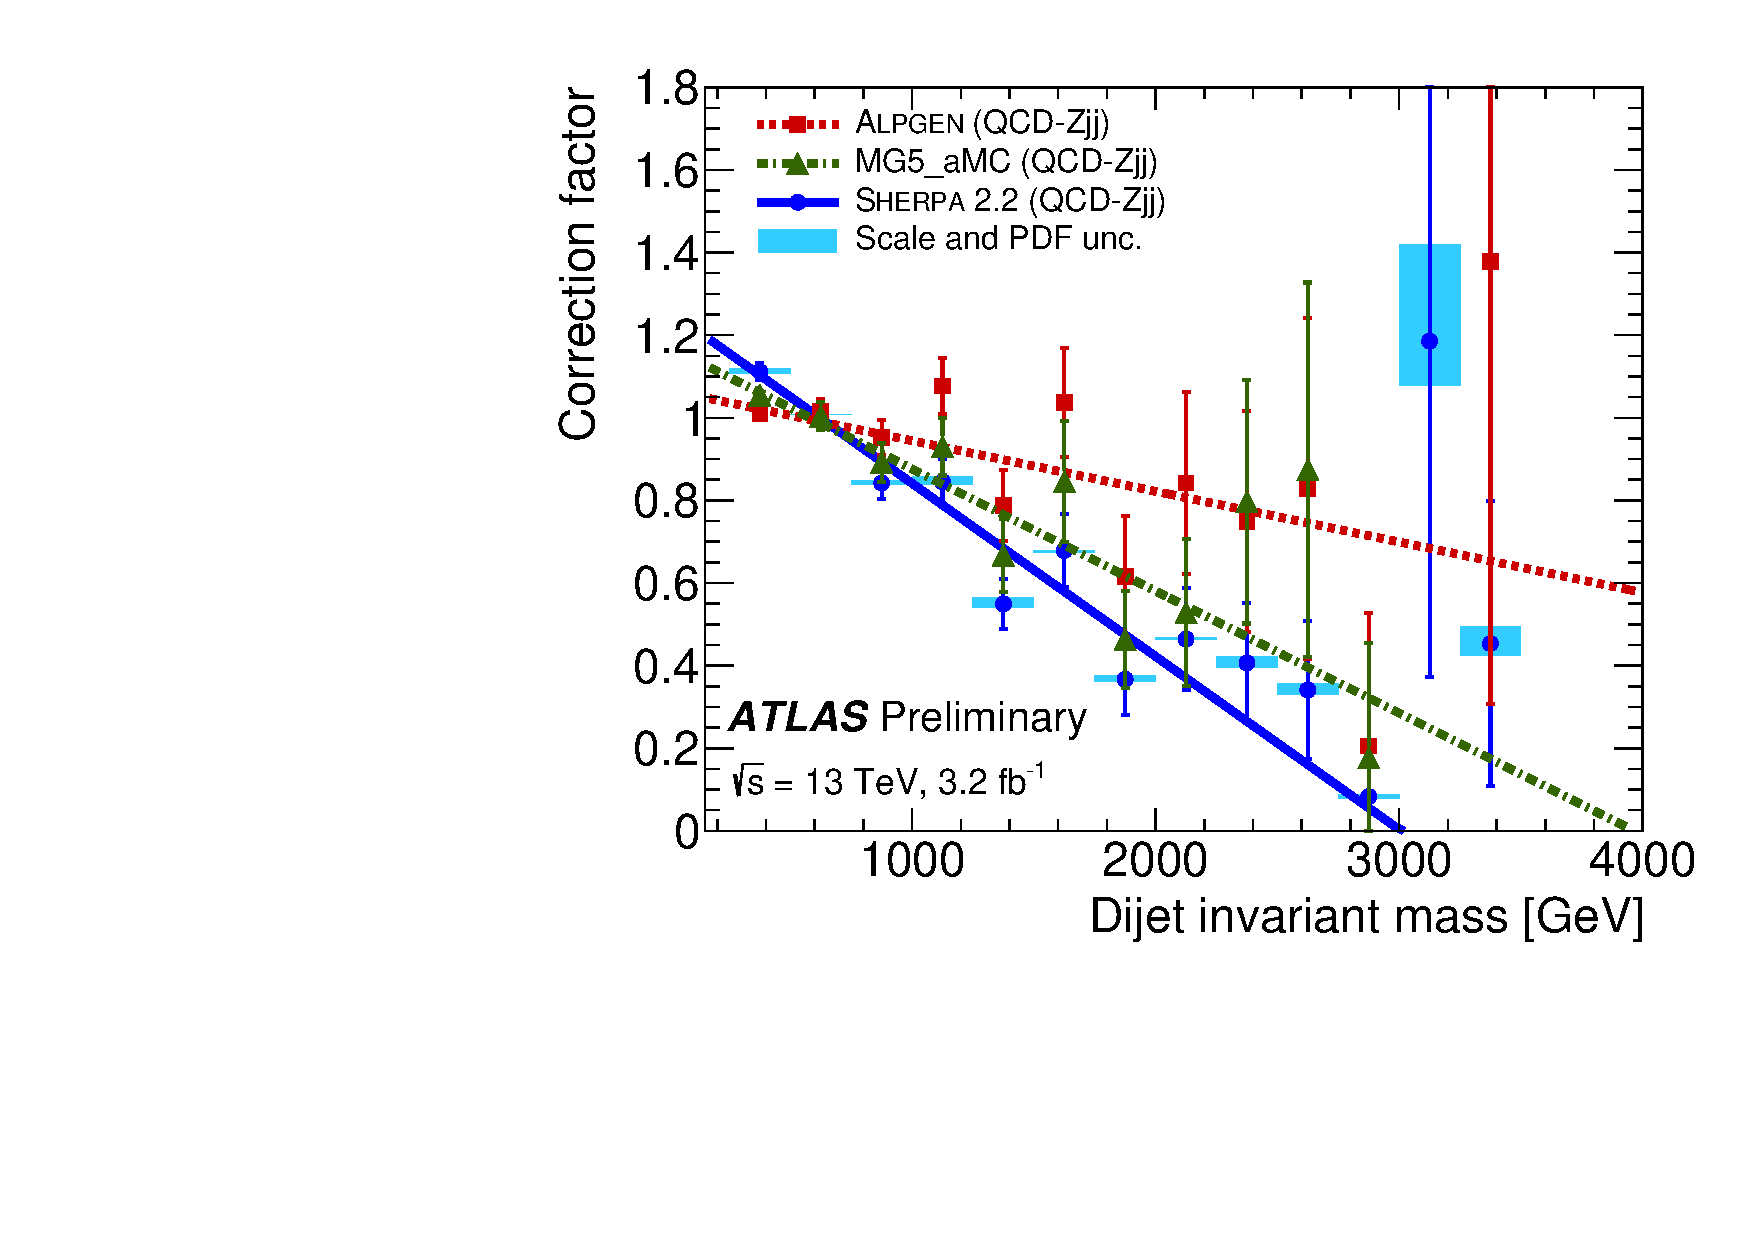
\includegraphics[width=.33\textwidth]{STDM-2016-09/fig_03a.pdf}
  \caption{$M_{jj}$ distribution.}
  \label{zjj-dijet-mismodeling}
\end{figure}

Figure~\ref{zjj-dijet-post-fit}.

\begin{figure}
  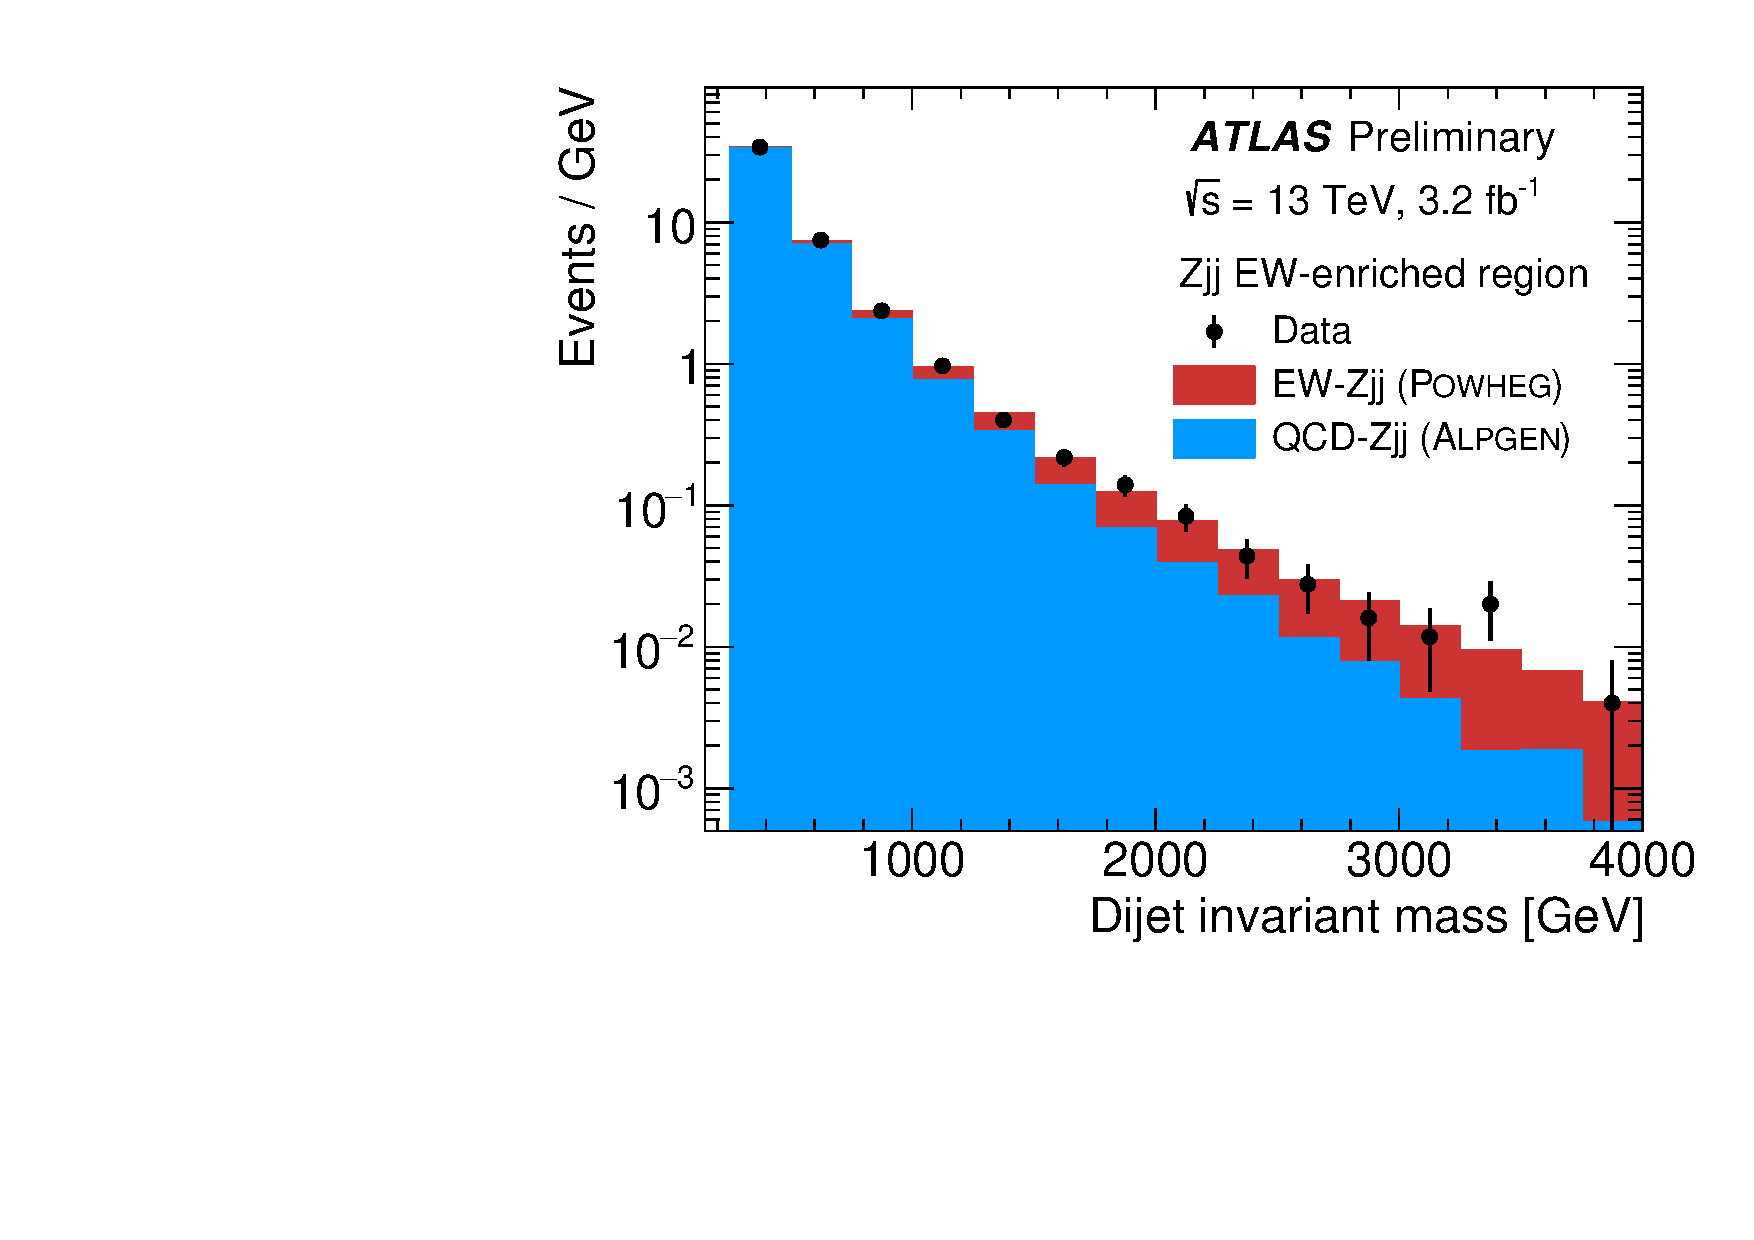
\includegraphics[width=.49\textwidth]{STDM-2016-09/fig_04a.pdf}
  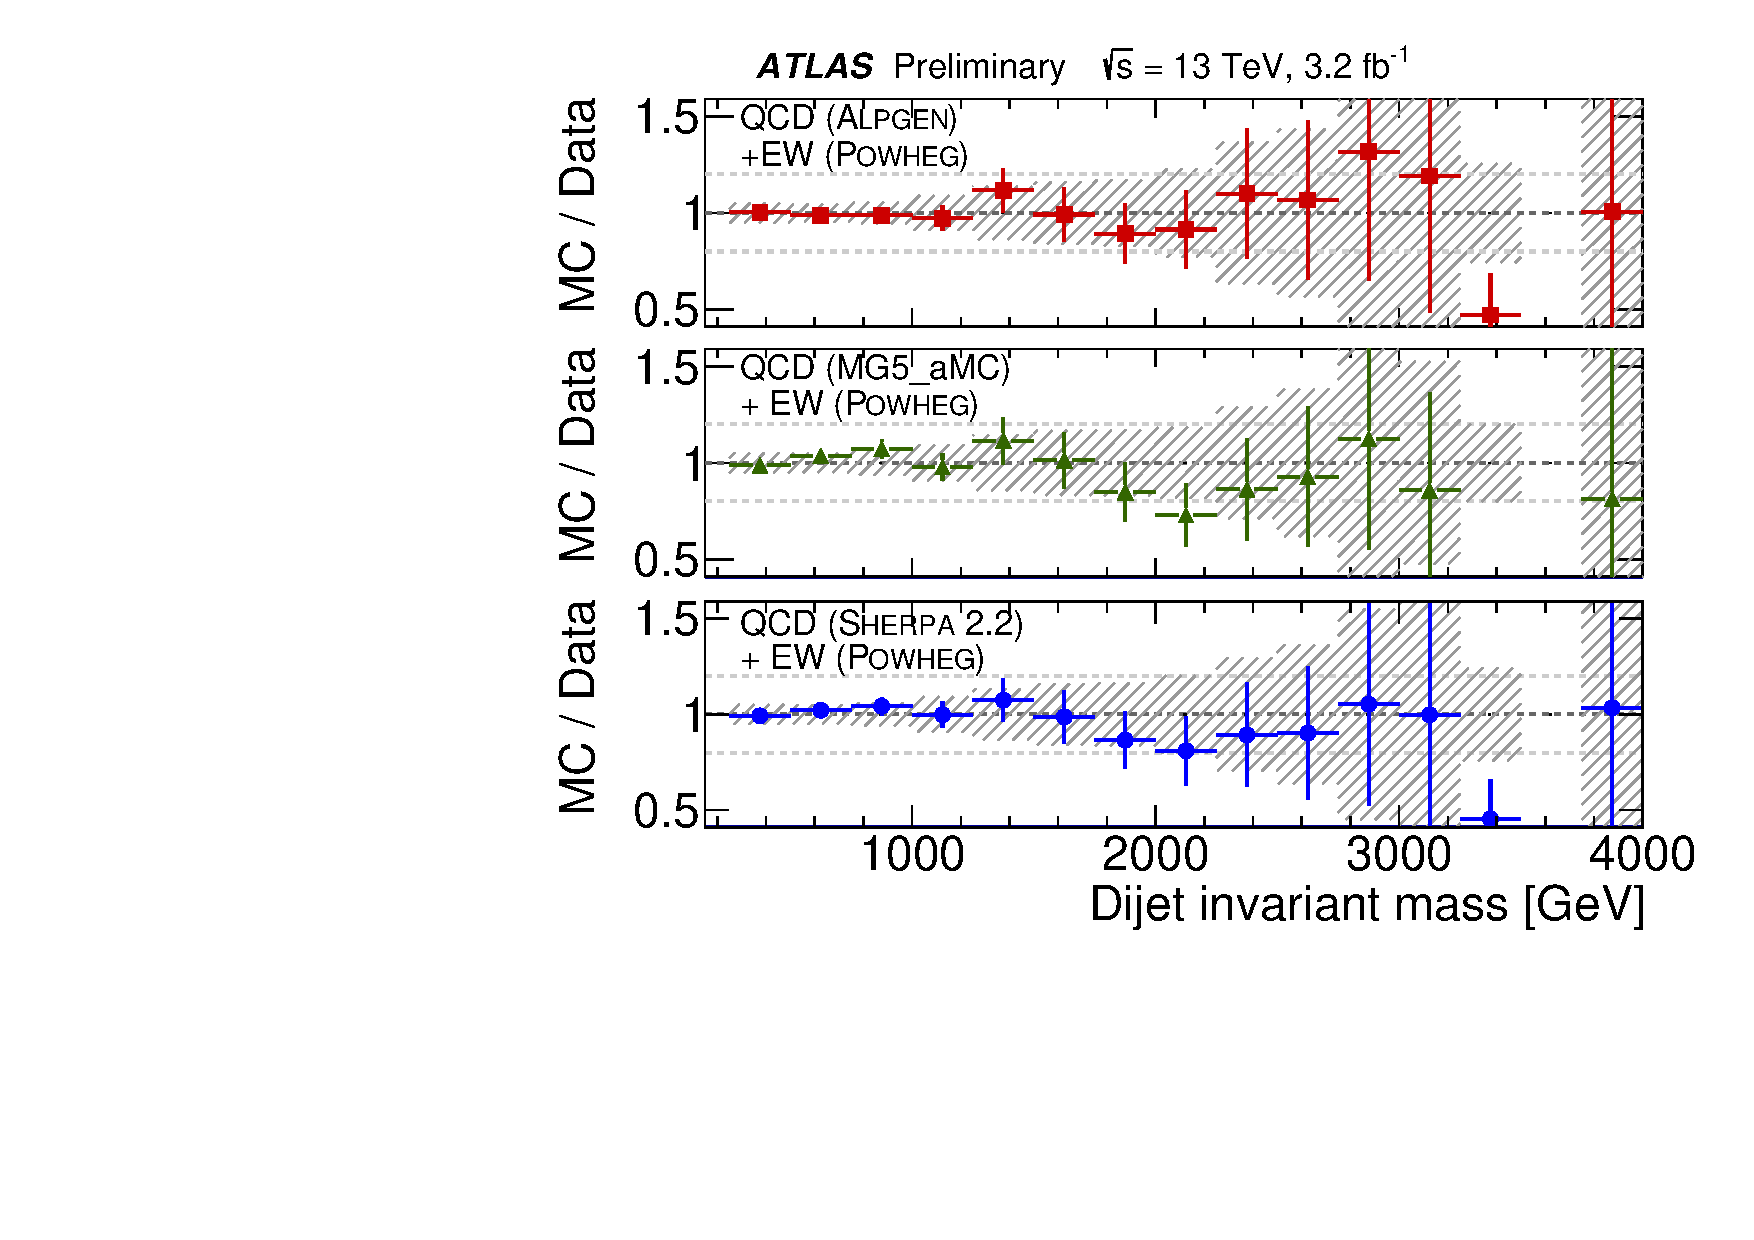
\includegraphics[width=.49\textwidth]{STDM-2016-09/fig_04b.pdf}
  \caption{Left: post-fit blah.}
  \label{zjj-dijet-post-fit}
\end{figure}

\section{Summary}

These results are consistent with Standard Model expectations.

Figure~\ref{zjj-wjj-summary-results}

\begin{figure}
  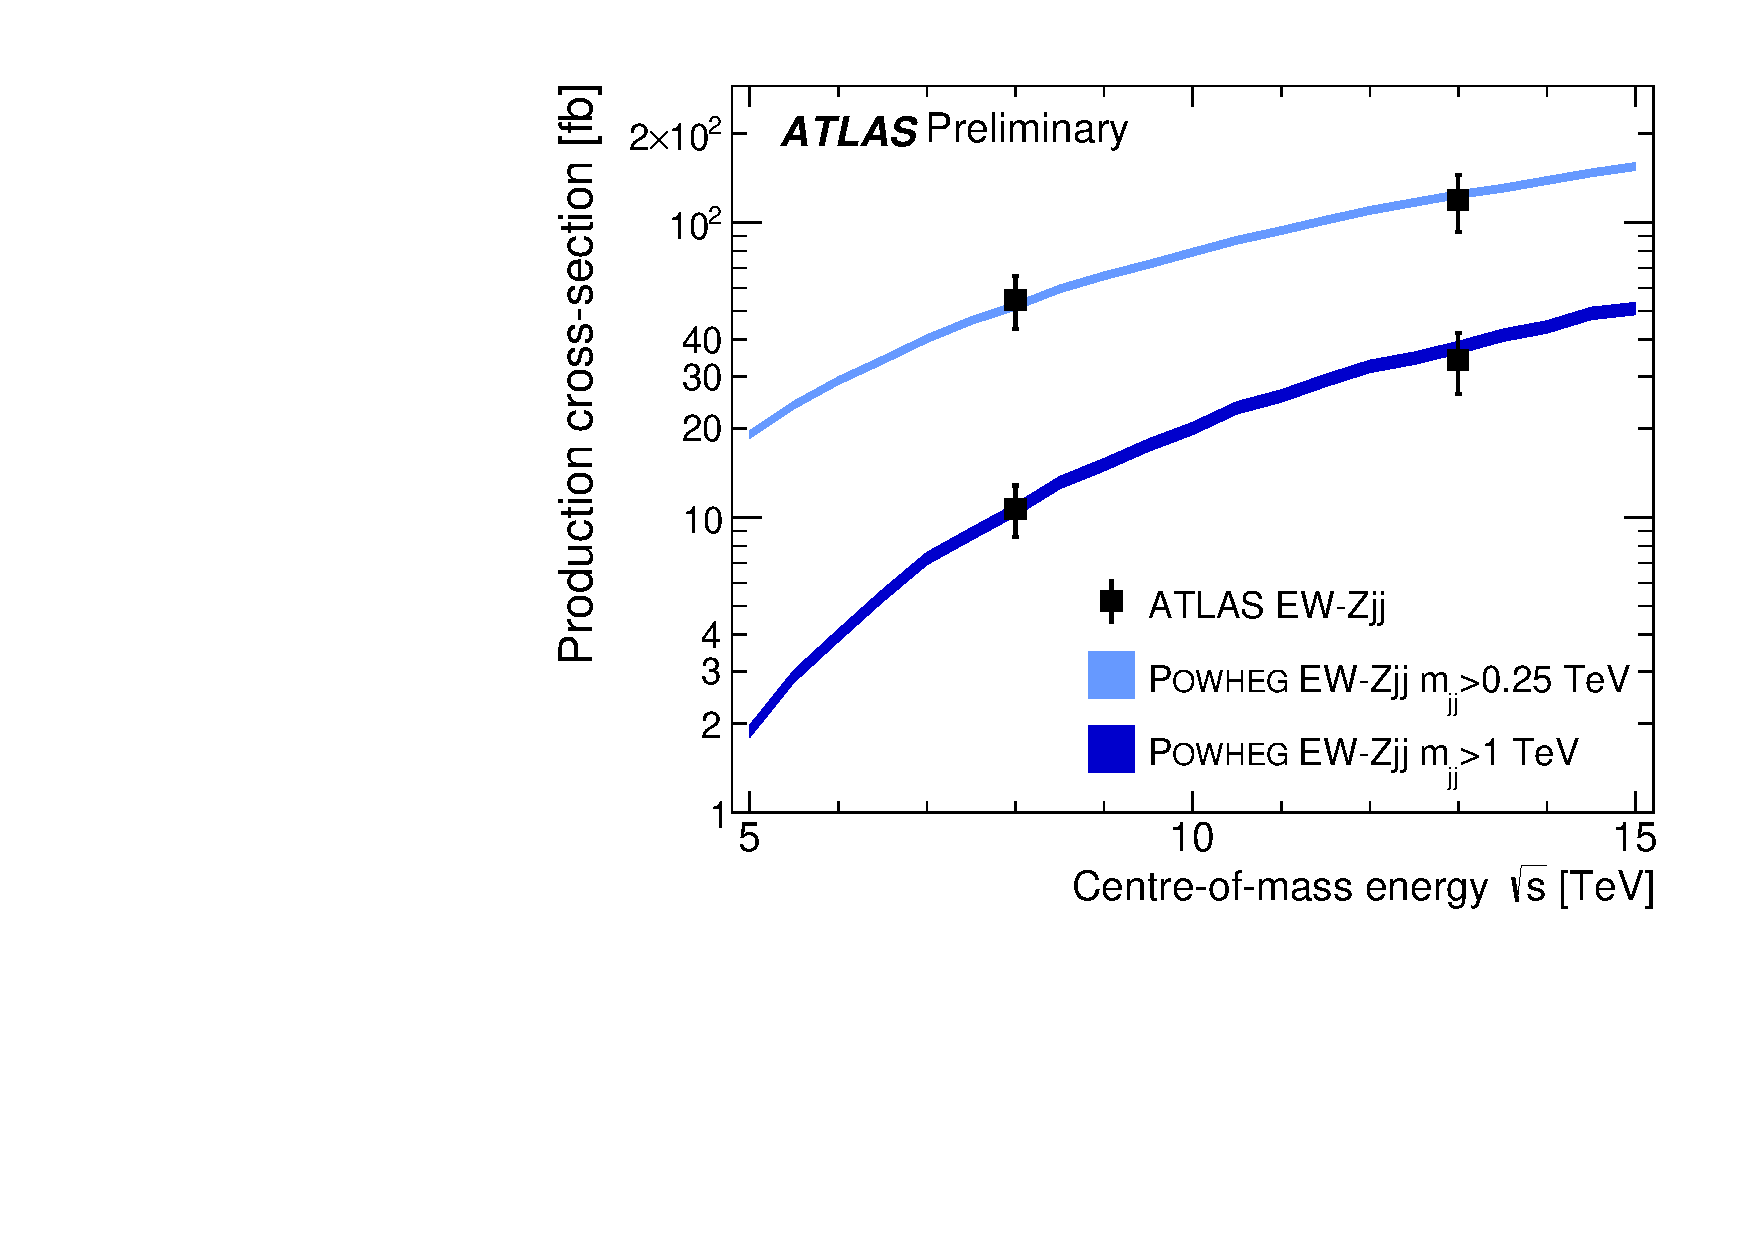
\includegraphics[width=.57\textwidth]{STDM-2016-09/fig_06.pdf}
  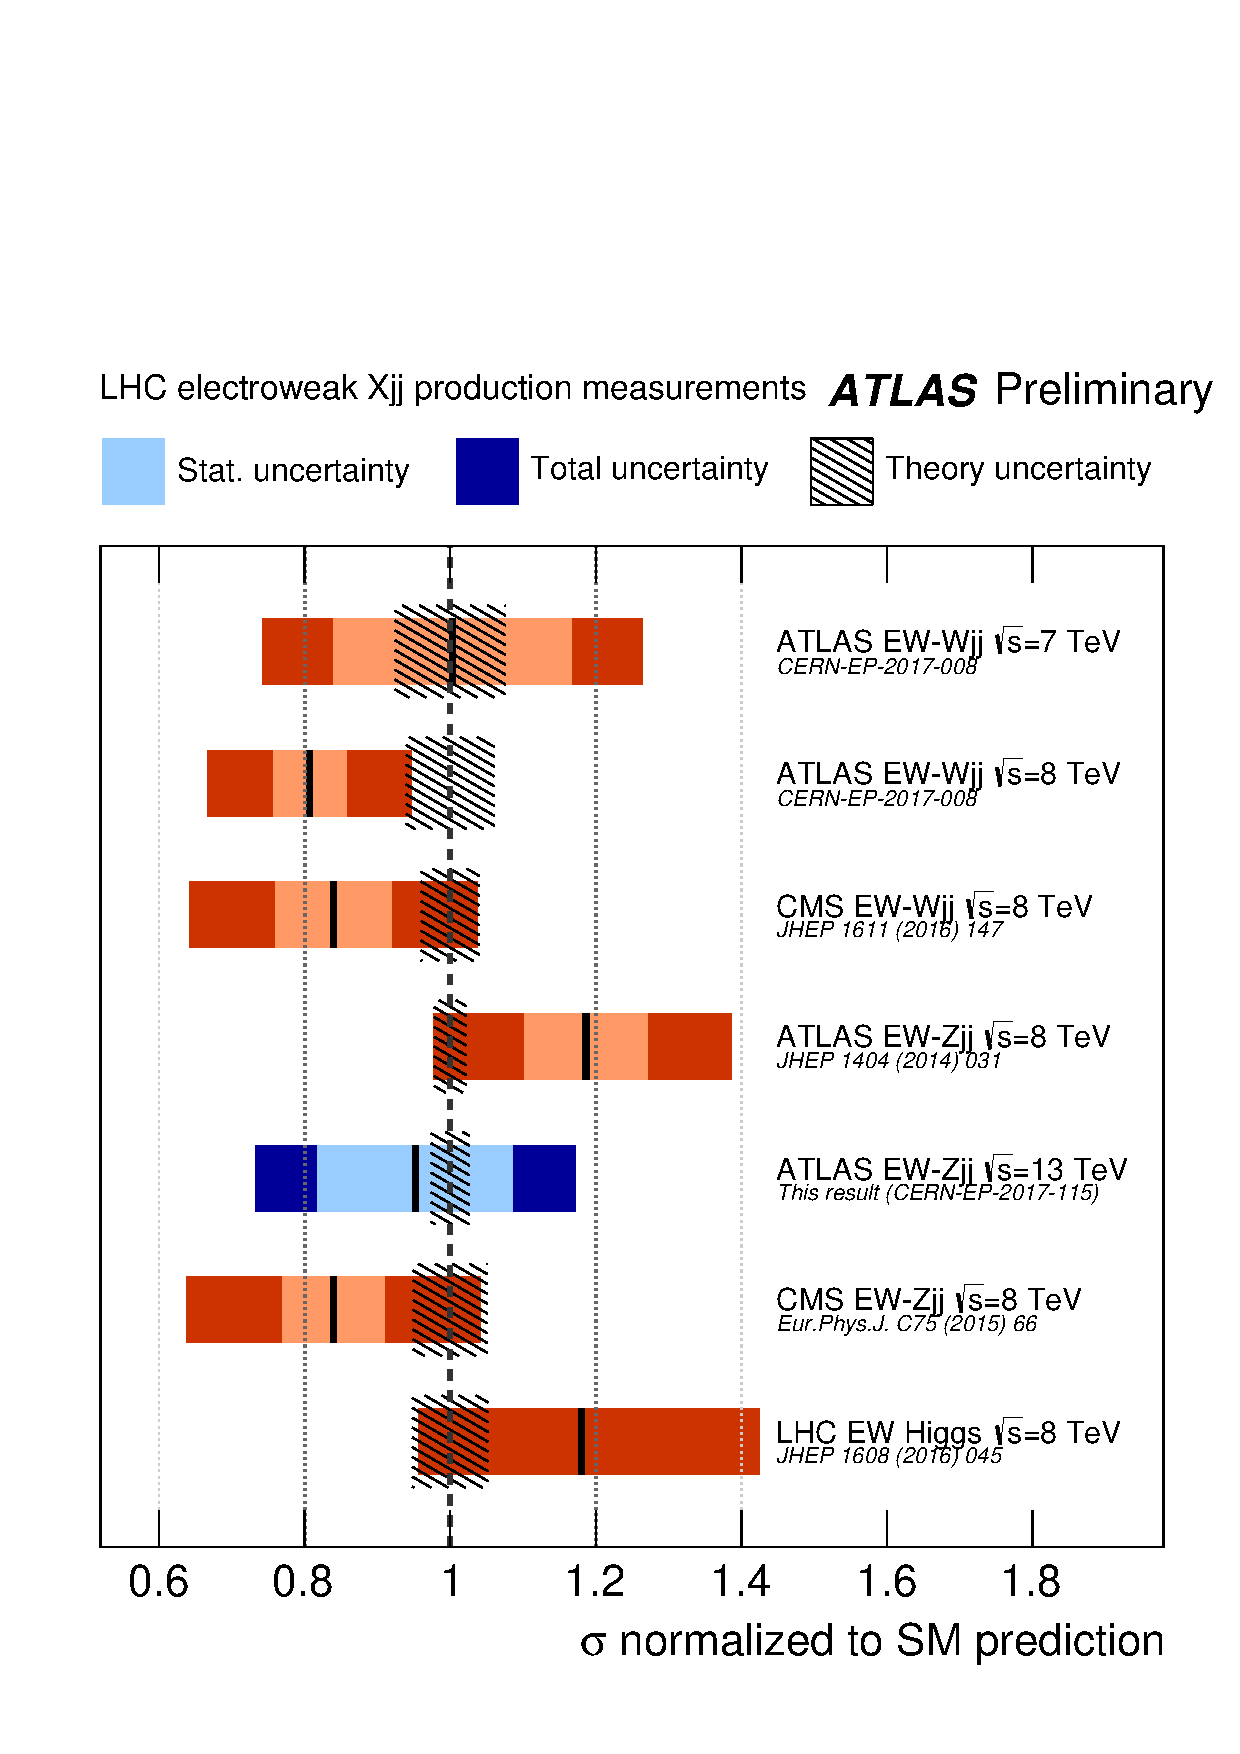
\includegraphics[width=.42\textwidth]{STDM-2016-09/fig_09.pdf}
  \caption{Left: \zjj measurement vs center-of-mass energy. Right: summary of electroweak \wjj and \zjj
measurements at ATLAS and CMS.}
  \label{zjj-wjj-summary-results}
\end{figure}


\bibliographystyle{JHEP}
\bibliography{my-bib-database}

\end{document}
